\documentclass[10pt]{beamer}
\beamertemplatenavigationsymbolsempty
\usecolortheme{beaver}
% \usetheme{Madrid}
\usefonttheme{professionalfonts}
\usepackage[utf8]{inputenc}
\usepackage[T1]{fontenc}
\usepackage{amsmath, amssymb, amsthm}
\usepackage[russian]{babel}
\usepackage[english]{babel}
\usepackage{hyperref}
\usepackage{algorithm, algorithmic}
\usepackage{graphicx}
\usepackage{booktabs}

\title{Computing upper and lower bounds on likelihoods in intractable networks}
\author{
Authors: Tommi S. Jaakola and Michael I. Jordan\\ 
\small Talk by Muhammadsharif Nabiev
}
\institute{Moscow Institute of Physics and Technology}
\date{2025}

\begin{document}

% ----------------------- Title -----------------------
\begin{frame}
  \titlepage
\end{frame}

% ---------------- Problem + Solution -----------------
\begin{frame}{Problem statement \& proposed solution}
\textbf{Problem.} In sigmoid and noisy-OR belief networks, exact likelihoods of partially observed variables can be intractable due to large cliques / exponential summations. \\
\medskip
\textbf{Goal.} Compute \emph{rigorous} upper and lower bounds on such likelihoods to form confidence intervals and enable decision-making without exact inference.

\textbf{Proposed solution.}
\begin{itemize}
  \item \textbf{Variational upper bounds} that factorize the intractable sum by introducing \emph{variational parameters} and exchanging minimization with marginalization (two-level networks).
  \item \textbf{Mean-field lower bounds} via Jensen’s inequality with tractable factorized $Q$ over unobserved nodes (generic networks).
\end{itemize}

\textbf{Networks covered.} Sigmoid belief networks and noisy-OR networks.
\end{frame}

% ---------------- Theoretic intro --------------------
\begin{frame}{Theoretic introduction}
\textbf{Graphical models.} DAG-structured joint $P(\mathbf{S}\mid\theta)=\prod_i P(S_i\mid \mathrm{pa}[i],\theta)$; exact inference by junction trees may be infeasible when cliques are large.

\begin{itemize}
  \item \textbf{Sigmoid network (binary $S_i$)}: 
  $P(S_i\!=\!1\mid \mathrm{pa}[i])=g\!\left(\sum_{j\in \mathrm{pa}[i]} \theta_{ij} S_j\right)$ with $g(x)=\tfrac{1}{1+e^{-x}}$.
  \item \textbf{Noisy-OR}: 
  $P(S_i\!=\!0\mid \mathrm{pa}[i])=\prod_{j\in\mathrm{pa}[i]} (1-q_{ij})^{S_j}
  = \exp\!\Big(-\sum_{j\in\mathrm{pa}[i]} \lambda_{ij} S_j\Big)$
  with $\lambda_{ij}=-\log(1-q_{ij})\ge 0$.
\end{itemize}

\textbf{Why bounds?} Exact confidence intervals for probabilities in general BNs are NP-hard; efficient \emph{bounds} can still be tight enough for practice.
\end{frame}

% --------------- Sigmoid UPPER: sketch ----------------
\begin{frame}{Upper bound for sigmoid network (two-level)}
\textbf{Setup.} Bipartite $L_2\!\to\!L_1$, observe all $\{S_i\}_{i\in L_1}$, hidden $\{S_j\}_{j\in L_2}$; write $y_i=2S_i-1\in\{-1,+1\}$ and let $\pi_j:=P(S_j=1)$.

\textbf{Sketch.}
\begin{enumerate}
  \item Insert the variational transform for the logistic:
  \[
  g(x)=\frac{1}{1+e^{-x}}=\min_{\xi\in[0,1]}\exp\!\big(-H(\xi)+\xi x\big),
  \]
  with binary entropy $H(\xi)=-\xi\log\xi-(1-\xi)\log(1-\xi)$.
  \item Apply to each observed node $g\big(y_i\sum_j \theta_{ij} S_j\big)$, collect terms by each hidden $S_j$; the augmented joint factorizes over $L_2$.
  \item \emph{Exchange minimization with marginalization} and sum out $S_j$ in closed form; finally minimize over $\boldsymbol{\xi}$.
\end{enumerate}
\end{frame}

% --------------- Sigmoid UPPER: result ----------------
\begin{frame}{Upper bound for sigmoid network (two-level)}
\textbf{Closed-form upper bound.}
\begin{multline*}
P(\{S_i\}_{i\in L_1}\mid \theta)
\;\le\; 
\min_{\boldsymbol{\xi}\in[0,1]^{|L_1|}}
\exp\!\Big(-\sum_{i\in L_1} H(\xi_i)\Big)\, \times \\
\prod_{j\in L_2}
\Big[
\pi_j \exp\!\Big(\sum_{i\in L_1} \xi_i\, y_i\, \theta_{ij}\Big)
+ (1-\pi_j)
\Big].
\end{multline*}

\textbf{Log form (for convex optimization).} Using $\log x=\min_{\alpha>0}\{\alpha x-\log\alpha-1\}$,
\[
\log P \;\le\;
-\sum_{i\in L_1} H(\xi_i)
+\sum_{j\in L_2}\log\!\Big[\pi_j e^{\sum_i \xi_i y_i \theta_{ij}}+(1-\pi_j)\Big]
\]
or equivalently with auxiliaries $\alpha_j>0$,
\[
\log P \;\le\;
-\sum_i H(\xi_i)
+\sum_j \alpha_j\!\Big[\pi_j e^{\sum_i \xi_i y_i \theta_{ij}}+(1-\pi_j)\Big]
-\sum_j(\log\alpha_j+1).
\]
\end{frame}

% --------------- Sigmoid LOWER: sketch (Jaakkola & Jordan narrative) ----------------
\begin{frame}{Lower bound for sigmoid network (generic)}
\textbf{Setup.} Evidence on $L_1$ with $y_i=2S_i-1$. Introduce a mean-field posterior over the hidden layer:
\[
Q(\mathbf{S}_{L_2})=\prod_{j\in L_2} \mu_j^{S_j}(1 - \mu_j)^{1-S_j} \approx\ P(\mathbf{S}_{L_2}\mid \mathbf{S}_{L_1}).
\]

\textbf{Sketch.}
\begin{enumerate}
  \item Apply Jensen’s inequality to the intractable sum over uninstantiated variables:
  \[
  \log P(\mathbf{S}_{L_1}) \;\ge\; \mathbb{E}_Q[\log P(\mathbf{S}_{L_1},\mathbf{S}_{L_2})] + H(Q).
  \]
  \item Decompose the joint under the sigmoid BN:
  \[
  \mathbb{E}_Q[\log P(\mathbf{S}_{L_1},\mathbf{S}_{L_2})]
  = \sum_{i\in L_1}\mathbb{E}_Q[\log P(S_i\!\mid\!\mathrm{pa}[i])]
    + \sum_{j\in L_2}\mathbb{E}_Q[\log P(S_j)].
  \]
  \item Under factorized $Q$, these expectations depend only on the means $\mu_j$; adjust $\{\mu_j\}$ to tighten the bound.
\end{enumerate}
\end{frame}

% --------------- Sigmoid LOWER: result (Jaakkola & Jordan narrative) ----------------
\begin{frame}{Lower bound for sigmoid network (generic)}
\textbf{Mean-field lower bound.}
\begin{multline*}
\log P(\{S_i\}_{i\in L_1}\mid \theta)
\;\ge\;
\sum_{i\in L_1}\mathbb{E}_Q\!\big[\log P(S_i\mid \mathrm{pa}[i];\theta)\big]
+ \\ \sum_{j\in L_2}\mathbb{E}_Q\!\big[\log P(S_j)\big]
+ H(Q)
\end{multline*}

\textbf{Notes (optimization).}
\begin{itemize}
  \item Maximize the RHS over $\boldsymbol{\mu}$; the bound is exact if $Q$ matches the true posterior.
  \item The accuracy of the bound   is governed by $\mathrm{KL}\!\left(Q\;\|\;P(\mathbf{S}_{L_2}\mid \mathbf{S}_{L_1})\right)$.
\end{itemize}
\end{frame}

% --------------- Noisy-OR UPPER: sketch (match paper) --------------
\begin{frame}{Upper bound for noisy-OR network (two-level)}
\textbf{Setup.} Bipartite $L_2\!\to\!L_1$. For child $i$ (no leak, as in the paper):
$$
P(S_i=1\mid \mathbf{S}_{L_2}) & = 1-\exp\Big(-\sum_j \lambda_{ij}S_j\Big),
$$
$$
P(S_i=0\mid \mathbf{S}_{L_2}) & = \exp\Big(-\sum_j \lambda_{ij}S_j\Big),
$$
with $\lambda_{ij}=-\log(1-q_{ij})\ge 0$ and $\pi_j:=P(S_j=1)$.

\textbf{Sketch.}
\begin{enumerate}
  \item Use the variational identity
  \[
  1-e^{-x}=\min_{\eta\ge 0}\exp\!\big(-\eta x - F(\eta)\big),\quad
  F(\eta)= -\eta\log\eta + (\eta+1)\log(\eta+1).
  \]
  \item Insert per observed node, regroup by parents ($L_2$): the augmented joint factorizes over $S_j$.
  \item Exchange the sum over $\mathbf{S}_{L_2}$ with the variational step to obtain a closed form in $\{\eta_i\}$, then (optionally) optimize them.
\end{enumerate}
\end{frame}

% --------------- Noisy-OR UPPER: result (match paper) --------------
\begin{frame}{Upper bound for noisy-OR network (two-level)}
\textbf{Closed-form upper bound.}
\begin{multline*}
P(\{S_i\}_{i\in L_1})
\;\le\;
\min_{\{\eta_i\ge 0\}} \left\{
\exp\!\Big(\!-\sum_{i\in L_1} S_i\,F(\eta_i)\Big) \times \\
\prod_{j\in L_2}
\Big[
\pi_j \exp\!\Big(\!-\sum_{i\in L_1} (S_i\eta_i+1-S_i)\lambda_{ij}\Big)
+ (1-\pi_j)
\Big] \right\}.
\end{multline*}

\medskip
\textbf{Log form.} 
Using $\log x=\min_{\alpha>0}\{\alpha x-\log\alpha-1\}$ and introducing auxiliaries $\{\alpha_j>0\}$,
\begin{multline*}
\log P
\;\le\;
-\sum_{i\in L_1} S_i\,F(\eta_i)
+ \\ \sum_{j\in L_2}\alpha_j
\Big[
\pi_j \exp\Big(-\sum_{i\in L_1} (S_i\eta_i+1-S_i)\lambda_{ij}\Big)
+ (1-\pi_j)
\Big] -\sum_{j\in L_2}(\log \alpha_j + 1).
\end{multline*}
\end{frame}


% --------------- Noisy-OR LOWER: sketch (matches paper style) --------------
\begin{frame}{Lower bound for noisy-OR network (generic)}
\textbf{Setup.} Reuse the same factorized $Q$ over the hidden parents and apply Jensen to $\log P(\mathbf{S}_{L_1})$ as before.

\textbf{Sketch.}
\begin{enumerate}
  \item Use the expansion $1-e^{-x}=\prod_{k} g(2^k x)$ with $g(u)=1/(1+e^{-u})$.
  \item Take logs and apply Jensen under $Q$ to the intractable terms.
  \item Use convexity to move expectations inside $\log(1+\cdot)$.
  \item Compute $\mathbb{E}_Q\!\left[e^{-2^k\sum_j \lambda_{ij}S_j}\right]
  =\prod_j\big(\mu_j e^{-2^k\lambda_{ij}}+(1-\mu_j)\big)$; for $S_i=0$ the term is exact: $-\sum_j \lambda_{ij}\mu_j$.
\end{enumerate}
\end{frame}

% --------------- Noisy-OR LOWER: result (identical to authors' Eq. 37) --------------
% --------------- Noisy-OR LOWER: result (closed-form + log form) --------------
\begin{frame}{Lower bound for noisy-OR network (generic)}
\small
\textbf{Closed-form.}
\begin{multline*}
P(\{S_i\}_{i\in L_1})
\ \ge\
e^{H(Q)}\,
\exp\!\Big(-\sum_{i:\,S_i=0}\sum_{j\in L_2}\lambda_{ij}\mu_j\Big)\, \\
\prod_{i:\,S_i=1}\ \prod_{k=0}^{\infty}
\Big(1+\prod_{j\in L_2}\big((1-\mu_j)+\mu_j e^{-2^k\lambda_{ij}}\big)\Big)^{-1}.
\end{multline*}

\textbf{Log form.}
\[
\begin{aligned}
\log P(\{S_i\}_{i\in L_1})
\ \ge\
&\sum_{i\in L_1}\sum_{k=0}^{\infty}
\Big[-\,S_i\,
\log\!\Big(1+\prod_{j\in L_2}\big(\mu_j e^{-2^k\lambda_{ij}}+(1-\mu_j)\big)\Big)\Big] \\
&\quad - \sum_{i\in L_1}(1-S_i)\sum_{j\in L_2}\lambda_{ij}\mu_j \;+\; H(Q).
\end{aligned}
\]
\end{frame}

% -------------------- Experiments --------------------
\begin{frame}{Experiments: sigmoid networks}
\small 
\textbf{Setup.} Complete bipartite $8\!\times\!8$ ($L_2\!\to\!L_1$). Weights $\theta_{ij}\sim\mathcal{N}(0,\sigma^2)$. Set $P(S_j=1)=1/2$ for all $j$. \\
\textbf{Metric.} Relative error in log-likelihood: $(\log P_{\text{bound}}/\log P)-1$ vs.\ inter-layer dependence
$\sigma_{\mathrm{std}}=\sqrt{\mathrm{Var}(P(S_i=1\mid \mathrm{pa}[i]))}$.

\begin{figure}
    \centering
    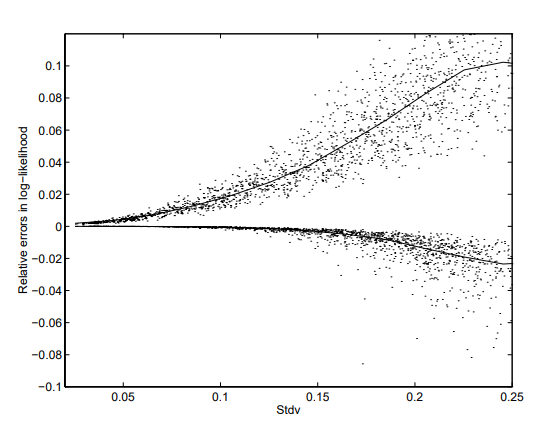
\includegraphics[width=0.6\linewidth]{sigmoid_bounds.png}
\end{figure}
Solid lines - median relative error. Upper bound degrades faster as coupling increases. Tight when layers are weakly coupled.
\end{frame}

\begin{frame}{Experiments: noisy-OR networks}
\textbf{Setup.} Complete bipartite $8\!\times\!8$; parameters $q_{ij}$ from a Dirichlet-controlled prior ($\text{Beta}(1, n)$ with $q_{ij} \sim n(1 - q_{ij})^{n-1}$). \\
\textbf{Metric.} Same relative log-likelihood error vs.\ $\sigma_{\mathrm{std}}$.
\begin{figure}
    \centering
    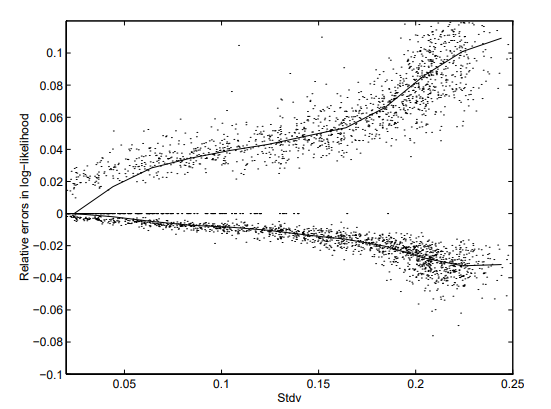
\includegraphics[width=0.6\linewidth]{noisyOR_bounds.png}
\end{figure}
Solid lines - median relative error. Upper bound exact for $S_i=0$. Lower bound a bit looser than sigmoid case. Upper bound deteriorates more quickly with stronger coupling.

\end{frame}

% ---------------------- Conclusion -------------------
\begin{frame}{Conclusion}
\begin{itemize}
  \item Variational upper bounds and lower bounds (generic) provide \emph{rigorous}, efficiently computable likelihood bracketing in otherwise intractable BN settings.
  \item For both sigmoid and noisy-OR, the approach yields practically tight bounds in weak-to-moderate coupling regimes and degrades gracefully with stronger dependence.
  \item Enables confidence intervals and principled decision-making without exact inference.
\end{itemize}
\end{frame}

\end{document}
